\documentclass{thesis}

%%
%% This part of your thesis is called the preamble.  It's a good idea
%% to put global definitions here.
%%

%% Permit the use of postscript figures within the document.
\usepackage{epsfig}

%% Use chicago style bibliography
\usepackage{chicago}

% Define your own fancy macro's for notation here.
\newcommand{\npclass}{$\cal{NP}$}

%%
%% One of the most important things you have to do in the preamble is
%% to tell who you are and what your thesis is about.
%%
\title{Working really hard for a few years and getting a master's degree}

\author{Your Name Here}
\mentor{Your Advisor's Name, Ph.D.}
\reader{One Committee Member, Ph.D.}
\readerThree{Another Committee Member, Ph.D.}
\readerFour{Still Another Member, Ph.D.}
\readerFive{Last Committee Member, Ph.D.}
\confDate{December 1999}
\makeCopyrightPage

%% You may have to change these but probably not.
\graduateDean{J. Larry Lyon, Ph.D.}
\schoolChair{Donald L. Gaitros, Ph.D.}

% Tell latex that there is no list of tables
\emptyLoT

\abstract{
This thesis is really cool and I should get a good job some day.  By the way,
the graduate school requires that this be no more than 150 words.
}

\begin{document}

%
% Now for the body of the thesis.  Here, we've split the thesis up into
% separate files for each individual chapter.
%

\pagenumbering{arabic}
	
% Introduction (What I'm trying to do)
\chapter{Introduction}

Lots of people write introductions \cite{whole-set}.  You can find 
very interesting introductions in lots of places 
\cite{booklet-full,inproceedings-full,article-full}.

Some readers may not understand how graduate school works.  
Firgure~\ref{how.to.graduate.fig} helps to explain the relationship between
the master's student and the graduate school.

\begin{figure}
\centerline{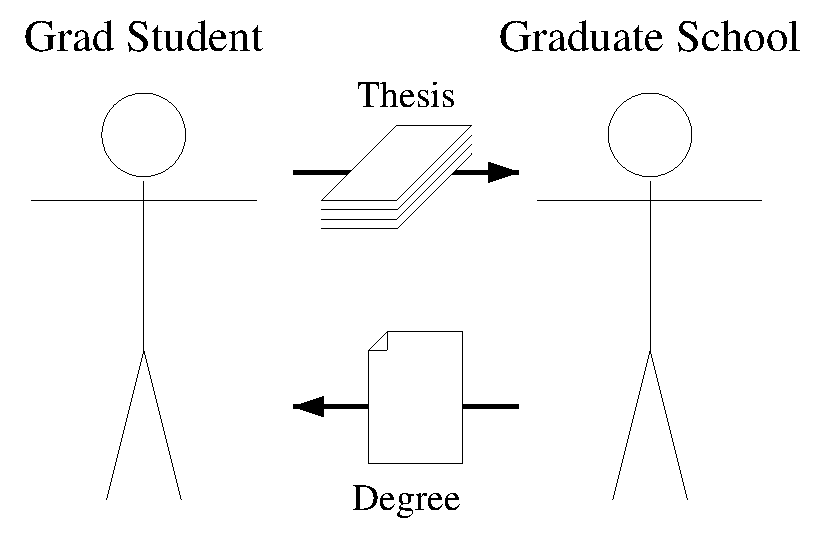
\includegraphics[height=0.34\textwidth,width=0.45\textwidth]{graduation.eps}}

\caption{In some cases, a thesis can be exchanged for an advanced degree.}

% This lets you refer to the figure by a unique identifier
\label{how.to.graduate.fig}
\end{figure}

Blah blah blah blah blah blah blah blah blah blah blah blah.
Blah blah blah blah blah blah blah blah blah blah blah blah.
Blah blah blah blah blah blah blah blah blah blah blah blah.
Blah blah blah blah blah blah blah blah blah blah blah blah.
Blah blah blah blah blah blah blah blah blah blah blah blah.
Blah blah blah blah blah blah blah blah blah blah blah blah.
Blah blah blah blah blah blah blah blah blah blah blah blah.
Blah blah blah blah blah blah blah blah blah blah blah blah.
Blah blah blah blah blah blah blah blah blah blah blah blah.
Blah blah blah blah blah blah blah blah blah blah blah blah.
Blah blah blah blah blah blah blah blah blah blah blah blah.
Blah blah blah blah blah blah blah blah blah blah blah blah.
Blah blah blah blah blah blah blah blah blah blah blah blah.
Blah blah blah blah blah blah blah blah blah blah blah blah.

\section{Stuff to think about}

Blah blah blah blah blah blah blah blah blah blah blah blah.
Blah blah blah blah blah blah blah blah blah blah blah blah.
Blah blah blah blah blah blah blah blah blah blah blah blah.
Blah blah blah blah blah blah blah blah blah blah blah blah.
Blah blah blah blah blah blah blah blah blah blah blah blah.
Blah blah blah blah blah blah blah blah blah blah blah blah.
Blah blah blah blah blah blah blah blah blah blah blah blah.
Blah blah blah blah blah blah blah blah blah blah blah blah.

\subsection{Really neat stuff}

Blah blah blah blah blah blah blah blah blah blah blah blah.
Blah blah blah blah blah blah blah blah blah blah blah blah.
Blah blah blah blah blah blah blah blah blah blah blah blah.
Blah blah blah blah blah blah blah blah blah blah blah blah.
Blah blah blah blah blah blah blah blah blah blah blah blah.
Blah blah blah blah blah blah blah blah blah blah blah blah.
Blah blah blah blah blah blah blah blah blah blah blah blah.
Blah blah blah blah blah blah blah blah blah blah blah blah.
Blah blah blah blah blah blah blah blah blah blah blah blah.
Blah blah blah blah blah blah blah blah blah blah blah blah.


\subsection{Boring stuff}

Blah blah blah blah blah blah blah blah blah blah blah blah.
Blah blah blah blah blah blah blah blah blah blah blah blah.
Blah blah blah blah blah blah blah blah blah blah blah blah.
Blah blah blah blah blah blah blah blah blah blah blah blah.
Blah blah blah blah blah blah blah blah blah blah blah blah.
Blah blah blah blah blah blah blah blah blah blah blah blah.
Blah blah blah blah blah blah blah blah blah blah blah blah.
Blah blah blah blah blah blah blah blah blah blah blah blah.
Blah blah blah blah blah blah blah blah blah blah blah blah.
Blah blah blah blah blah blah blah blah blah blah blah blah.

\section{Stuff to ignore}

Blah blah blah blah blah blah blah blah blah blah blah blah.
Blah blah blah blah blah blah blah blah blah blah blah blah.
Blah blah blah blah blah blah blah blah blah blah blah blah.
Blah blah blah blah blah blah blah blah blah blah blah blah.
Blah blah blah blah blah blah blah blah blah blah blah blah.
Blah blah blah blah blah blah blah blah blah blah blah blah.
Blah blah blah blah blah blah blah blah blah blah blah blah.
Blah blah blah blah blah blah blah blah blah blah blah blah.
Blah blah blah blah blah blah blah blah blah blah blah blah.
Blah blah blah blah blah blah blah blah blah blah blah blah.


% Related work (Stuff other people did)
\chapter{Related Work}

Other people are really smart.

	
% Prototype Implementation (Stuff I did)
\chapter{Design and Implementation}

I'm a little smart too.


% Experimental results (How it did)
\chapter{Experimental Results}

See, it really works.


% Conclusion 
\chapter{Summary}

Well, I didn't do everything I wanted to, but I made a good start.  If someone
else wants to work on this for a little while, that would be great.


% This line says how to format the bibliography
\bibliographystyle{chicago}

% This line says where to get the bibliography entries.
\bibliography{references}
	
\end{document}
